
%
% حق نشر 1390-1402 دانش پژوهان ققنوس
% حقوق این اثر محفوظ است.
% 
% استفاده مجدد از متن و یا نتایج این اثر در هر شکل غیر قانونی است مگر اینکه متن حق
% نشر بالا در ابتدای تمامی مستندهای و یا برنامه‌های به دست آمده از این اثر
% بازنویسی شود. این کار باید برای تمامی مستندها، متنهای تبلیغاتی برنامه‌های
% کاربردی و سایر مواردی که از این اثر به دست می‌آید مندرج شده و در قسمت تقدیر از
% صاحب این اثر نام برده شود.
% 
% نام گروه دانش پژوهان ققنوس ممکن است در محصولات دست آمده شده از این اثر درج
% نشود که در این حالت با مطالبی که در بالا اورده شده در تضاد نیست. برای اطلاع
% بیشتر در مورد حق نشر آدرس زیر مراجعه کنید:
% 
% http://dpq.co.ir/licence
%
\chapter{نصب}
% در این فصل نشان داده می‌شود که چگونه باید این نرم‌افزار را نصب کرد، و برای
% تولید مستند از آن استفاده کرد.\cite{surhone2010doxygen}
 
برای نصب \lr{Doxygen} و \lr{Doxywizard} ابتدا باید آن‌ها را دریافت کنید. این
برنامه‌ها کاملا رایگان هستند.
در واقع \lr{Doxygen} یک نرم‌افزار متن باز\LTRfootnote{Open Source} است. متن
این برنامه و همچنین پرونده‌ی قابل اجرای آن را می‌توان از آدرس
\url{http://www.doxygen.org/download.html} 
دریافت کرد. برای نصب این برنامه می‌توانید متن آن را دریافت کنید و سپس آن را
روی سیستم خود ترجمه (کامپایل) کنید و از آن استفاده کنید. روش دیگر هم این است
که از برنامه‌های ترجمه شده و قابل اجرایی که روی آدرس ذکر شده قرار دارد
استفاده کنید. در این کتاب فقط روش دوم را شرح می‌دهیم، چون روش عمومی‌تری است.

% در این قسمت نحوه‌ی نصب بر روی سیستم عامل اوپن سوزی شرح داده می شود. به دلیل اینکه در اوپن سوزی
% روشی ساده با گرافیکی کاربرپسند برای نصب برنامه ها وجود دارد، نصب روی این سیستم عامل را به طور جداگانه
% علاوه بر سیستم عامل‌های لینوکسی آورده‌ایم.
% محمد هادی منصوری ۹۰/۳/۳
\section{\lr{OpenSUSE}}

اگرچه دستورالعمل مربوط به نصب \lr{Doxygen} روی سیستم عامل‌های لینوکسی برای سیستم
عامل \lr{OpenSUSE} هم قابل استفاده است، اما سیستم عامل \lr{OpenSUSE} روشی
گرافیکی ساده و کاربرپسندی برای نصب برنامه‌ها دارد.
در این سیستم عامل مدیریت گرافیکی \lr{YaST} امکانات مناسبی برای مدیریت قسمت‌های
مختلف سیستم فراهم آورده است.
از جمله‌ی این امکانات مدیریت مخزن‌ها\footnote{\lr{Repository}}و مدیریت
نرم‌افزارها\footnote{\lr{Software Management}} است.

برای نصب \lr{Doxygen}، ابتدا باید به اینترنت وصل باشید. سپس از طریق منوی شروع در
\lr{OpenSUSE} که با علامت 
\includegraphics[width=0.5cm]{image/opensuse} نشان
داده می‌شودبرنامه‌ی \lr{YaST} را اجرا کنید. سپس قسمت \lr{Software Management} را
انتخاب کنید. پس از اینکه ابزار مدیریت نرم‌افزارها باز شد، در قسمت جستجو، کلمه‌ی
\lr{doxy} را جستجو کنید. در فهرستی که از نتیجه‌ی جستجو نشان داده می‌شود
برنامه‌های \lr{doxygen} و \lr{doxywizard} را به حالت انتخاب در آورید، و سپس
دکمه‌ی تایید را بزنید تا سیستم شروع به نصب برنامه‌ها کند. هر کدام از این
برنامه‌ها که قبلا روی سیستم شما نصب شده باشند به حالت انتخاب شده هستند و نیازی
به نصب آن ندارید. البته ممکن است که بخواهید آن برنامه را به‌روز کنید. تصویر
\ref{image/install/OpenSUSE/setup} را مشاهده کنید.

\begin{figure}
 \centering
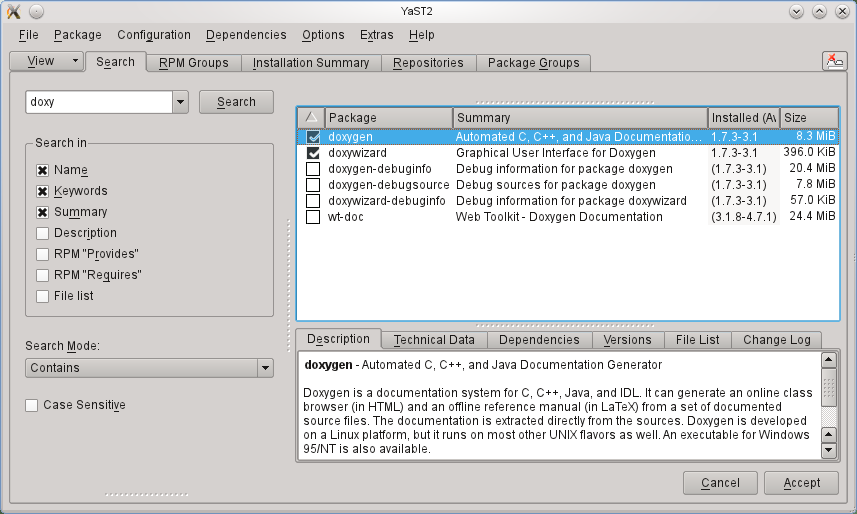
\includegraphics[width=0.75\textwidth]{image/install/OpenSUSE/setup}
\caption[پنجره‌ی نصب برنامه‌ها در سیستم عامل \lr{OpenSUSE}.]{
پنجره‌ی نصب برنامه‌ها در سیستم عامل \lr{OpenSUSE}. پس از جستجوی نام ابزار مورد
نظر خود، آن‌ها را انتخاب کرده و سپس شروع به نصب کنید.
}
\label{image/install/OpenSUSE/setup}
\end{figure}

در صورتی که \lr{doxygen} یا \lr{doxywizard} در نتایج جستجو مشاهده نشد، احتمالا
مخزن مربوط به این نرم‌افزارها در فهرست مخزن‌های سیستم شما وجود ندارد و باید آن
را اضافه کنید. برای این کار ابتدا آدرس یک مخزن که این ابراز را دارد پیدا کنید
سپس در \lr{YaST} به قسمت \lr{Software Repositories} رفته و این آدرس را به فهرست
مخزن‌های سیستم اضافه کنید. پس از آن دوباره نام ابزارها را جستجو کنید و آن‌ها را
نصب کنید.


% در این قسمت نحوه‌ی نصب، روی سیستم عامل های لینوکسی شرح داده می شود.
% محمد هادی منصوری ۹۰/۳/۲
%
% حق نشر 1390-1402 دانش پژوهان ققنوس
% حقوق این اثر محفوظ است.
% 
% استفاده مجدد از متن و یا نتایج این اثر در هر شکل غیر قانونی است مگر اینکه متن حق
% نشر بالا در ابتدای تمامی مستندهای و یا برنامه‌های به دست آمده از این اثر
% بازنویسی شود. این کار باید برای تمامی مستندها، متنهای تبلیغاتی برنامه‌های
% کاربردی و سایر مواردی که از این اثر به دست می‌آید مندرج شده و در قسمت تقدیر از
% صاحب این اثر نام برده شود.
% 
% نام گروه دانش پژوهان ققنوس ممکن است در محصولات دست آمده شده از این اثر درج
% نشود که در این حالت با مطالبی که در بالا اورده شده در تضاد نیست. برای اطلاع
% بیشتر در مورد حق نشر آدرس زیر مراجعه کنید:
% 
% http://dpq.co.ir/licence
%
\section{لینوکس}
\label{install/linux}

\begin{sloppypar}
برای نصب \lr{Doxygen} روی سیستم عامل‌های لینوکسی نیاز به توزیع دودویی مناسب برای سیستم عامل خود دارید. از آدرس 
\url{http://www.doxygen.org/download.html}
 می‌توانید توزیع مناسب را دریافت کنید. پس از دریافت توزیع مناسب، با دستورات زیر می‌توان \lr{Doxygen} را نصب کرد. 
معمولا بین پرونده‌های دریافت شده، پرونده‌ای به نام \lr{configure} وجود دارد. این پرونده حاوی دستورات خط فرمان (دستورات شل) برای 
پیکربندی اولیه است. دستورات زیر پیکربندی اولیه را انجام داده و برنامه را نصب می‌کند.
\end{sloppypar}
\begin{latin}
\lstset{language=C++}  
\begin{lstlisting}[frame=single] 
./configure
make install
\end{lstlisting}
\end{latin}
%\begin{flushleft}
%\lr{./configure} \\
%\lr{make install}
%\end{flushleft}
برای نصب مستندات و مثال‌ها دستور زیر را اجرا کنید.
\begin{latin}
\lstset{language=C++}  
\begin{lstlisting}[frame=single] 
make install_docs
\end{lstlisting}
\end{latin}
%\begin{flushleft}
%\lr{make install\_docs}
%\end{flushleft}
پرونده‌های اجرایی در مسیر 
\lr{<prefix>/bin}
 و مستندات و مثال‌ها در مسیر 
\lr{<docdir>/doxygen}
  نصب می‌شوند.

\begin{sloppypar}
به صورت پیش‌فرض 
\lr{<prefix>}
 به آدرس 
\lr{usr/local}
 اشاره دارد، اما می‌توان آن را با تغییر پارامتر 
\lr{--prefix}
 در پرونده‌ی \lr{configure} تغییر داد. 
\lr{<docdir>}
 نیز به صورت پیش‌فرض به آدرس 
\lr{<prefix>/share/doc/packages}
 اشاره دارد که این آدرس را نیز می‌توان با تغییر پارامتر 
\lr{--doxdir}
 در پرونده‌ی \lr{configure} عوض کرد.
\end{sloppypar}

در صورتی که از بسته‌های \lr{RPM} یا \lr{DEP} استفاده می‌کنید، همان روند استاندارد 
نصب را دنبال کنید که برای این بسته‌ها مورد نیاز است.


% در این قسمت نحوه‌ی نصب DoxyGen روی سیستم عامل ویندوز توضیح داده شده است.
% محمد هادی منصوری. ۹۰/۳/۱
%
% حق نشر 1390-1402 دانش پژوهان ققنوس
% حقوق این اثر محفوظ است.
% 
% استفاده مجدد از متن و یا نتایج این اثر در هر شکل غیر قانونی است مگر اینکه متن حق
% نشر بالا در ابتدای تمامی مستندهای و یا برنامه‌های به دست آمده از این اثر
% بازنویسی شود. این کار باید برای تمامی مستندها، متنهای تبلیغاتی برنامه‌های
% کاربردی و سایر مواردی که از این اثر به دست می‌آید مندرج شده و در قسمت تقدیر از
% صاحب این اثر نام برده شود.
% 
% نام گروه دانش پژوهان ققنوس ممکن است در محصولات دست آمده شده از این اثر درج
% نشود که در این حالت با مطالبی که در بالا اورده شده در تضاد نیست. برای اطلاع
% بیشتر در مورد حق نشر آدرس زیر مراجعه کنید:
% 
% http://dpq.co.ir/licence
%
\section{ویندوز}

در آدرس
\url{http://www.doxygen.org/download.html} 
یک برنامه‌ی اجرایی برای نصب نسخه‌ی ویندوزی وجود دارد. این برنامه به صورت یک
مجموعه کامل قابل نصب است و نصب آن بسیار ساده است.
کافی است پنجره‌های محاوره‌ای را دنبال کنید.



در هنگام نصب در یکی از مراحل از کاربر خواسته می‌شود موارد لازم برای نصب را تعیین کند. 
تصویر \ref{پنجره_نصب_روی_ویندوز} را ببینید. در این مرحله 
فهرستی از ابزارهایی که نصب می‌شودقرار داده شده است. 
همانگونه که در تصویر \ref{پنجره_نصب_روی_ویندوز} دیده می‌شود یکی از ابزارها، \lr{Doxywizard} است. 
به این ترتیب می‌توان در نسخه‌ی ویندوزی، هر دو ابزار \lr{Doxygen} و \lr{Doxywizard} را نصب کرد.

\begin{figure}
\centering
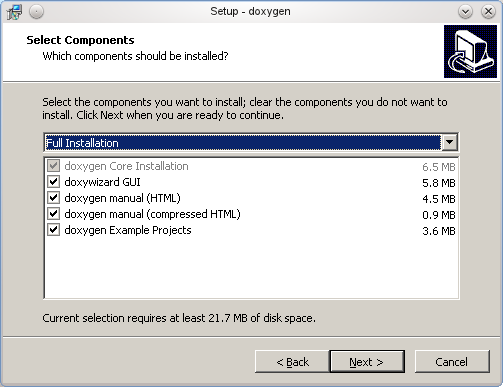
\includegraphics[width=0.75\textwidth]{image/windows_setup}
\caption[
پنجره‌ی محاوره‌ای نصب
{\lr{Doxygen}}
 روی ویندوز
]{
پنجره‌ی محاوره‌ای نصب
{\lr{Doxygen}}
 روی ویندوز. در این پنجره فهرستی از مواردی که باید نصب شود قرار دارد.
}
\label{پنجره_نصب_روی_ویندوز}
\end{figure}

توصیه می شود که بعد از نصب،
\lr{GraphViz} 
(نسخه‌ی ۲/۸ یا جدیدتر) را هم دریافت کرده و نصب کنید.
\lr{Doxygen}
 می تواند از ابزار
\lr{dot}
 مربوط به بسته‌ی
\lr{GraphViz}
، برای تولید بهتر دیاگرام ها استفاده کند.
% تنظیم \lr{HAVE\_DOT} در پرونده‌ی پیکربندی را مشاهده کنید.

اگر می‌خواهید پرونده‌های فشرده‌ی \lr{HTML} تولید کنید، نیاز به 
\lr{Microsoft HTML help} 
دارید. این ابزار را می‌توانید از آدرس 
\url{http://msdn.microsoft.com/en-us/library/ms670169}
 دریافت کنید.
%(تنظیم \lr{GENERATE\_HTMLHELP} را در پرونده‌ی پیکربندی مشاهده کنید)،

اگر می‌خواهید پرونده‌های فشرده‌ی \lr{Qt} را تولید کنید، نیاز به \lr{qhelpgenerator} دارید که قسمتی از \lr{Qt} 
 است. \lr{Qt} را می‌توانید از آدرس 
\url{http://qt.nokia.com/downloads/}
دریافت کنید.

به منظور تولید خروجی \lr{PDF}، یا استفاده از فرمول‌های خاص، احتیاج به نصب
\lr{LaTeX} و \lr{Ghostscript} دارید.
برای \lr{LaTex} چند توزیع وجود دارد. از جمله موارد معروف که باید با \lr{doxygen}
کار کنند \lr{MikTex} و \lr{XemTex} است\footnote{متاسفانه تولید مستند در قالب
\lr{LaTeX} با استفاده از \lr{Doxygen} برای مستندات به زبان فارسی با مشکلاتی
روبروست}.
\lr{Ghostscript} 
 را می‌توان از آدرس
\url{http://sourceforge.net/projects/ghostscript/} 
 دریافت کرد.

پس از نصب \lr{LaTex} و \lr{Ghostscript} باید مطمئن شوید که ابزارهای
\lr{latex.exe}، \lr{pdflatex.exe} و \lr{gswin32c.exe} در مسیر جستجوی دستورات خط
فرمان قرار دارند. در صورتی که از این موضوع مطمئن نیستید دستورالعمل زیر را دنبال
کنید و دستورات را در خط فرمان اجرا کنید تا ببینید به درستی کار می‌کنند یا نه.

از صفحه‌ی اصلی ویندوز روی \lr{My Computer} کلیک راست کرده و گزینه‌ی
\lr{Properties} را انتخاب کنید.
 در پنجره‌ای که ظاهر می‌شود زبانه‌ی \lr{Advanced} را انتخاب کنید. سپس دکمه‌ی
 \lr{Environment Variables} را کلیک کنید.
 در پنجره‌ای که ظاهر می‌شود متغیر \lr{Path} را انتخاب کرده و دکمه‌ی \lr{Edit} را
 کلیک کنید.
 سپس مسیرهای مربوط به ابزارهای گفته شده را در صورتی که وجود نداشت، در این قسمت
 اضافه کنید.
 مسیرهای مختلف با استفاده از علامت نقطه ویرگول از هم جدا می‌شوند. مثلا
\lr{C:\textbackslash Program Files;C:\textbackslash Winnt;C:\textbackslash
Winnt\textbackslash System32}.

پس از انجام کارهای گفته شده نرم‌افزار \lr{Doxygen} نصب شده و آماده استفاده است.
